% Created by tikzDevice version 0.12.5 on 2023-10-05 04:11:54
% !TEX encoding = UTF-8 Unicode
\definecolor{triplet}{HTML}{E69F00}
\definecolor{mar-sum}{HTML}{009E73}
\definecolor{mar-max}{HTML}{CC79A7}
\definecolor{color1}{HTML}{CC9966}
\definecolor{color2}{HTML}{99CCFF}
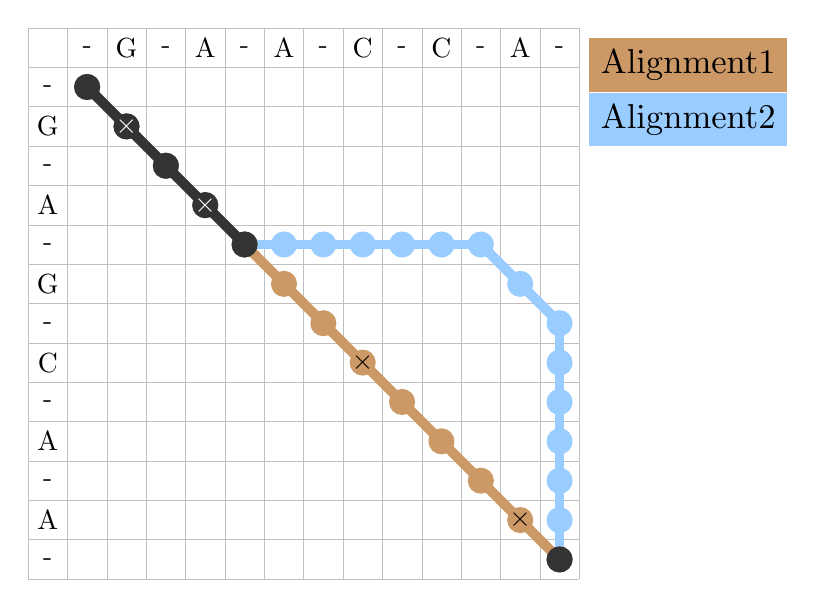
\begin{tikzpicture}[dot/.style={circle, minimum size=2.5mm}, box/.style={rectangle, minimum size = 3.5cm, anchor = north west}]
\draw[very thin, color = gray!50, step = 0.5] (0,0) grid (7, 7);
\node at (0.25,6.25) {-};
\node at (0.25,5.75) {G};
\node at (0.25,5.25) {-};
\node at (0.25,4.75) {A};
\node at (0.25,4.25) {-};
\node at (0.25,3.75) {G};
\node at (0.25,3.25) {-};
\node at (0.25,2.75) {C};
\node at (0.25,2.25) {-};
\node at (0.25,1.75) {A};
\node at (0.25,1.25) {-};
\node at (0.25,0.75) {A};
\node at (0.25,0.25) {-};
\node at (0.75,6.75) {-};
\node at (1.25,6.75) {G};
\node at (1.75,6.75) {-};
\node at (2.25,6.75) {A};
\node at (2.75,6.75) {-};
\node at (3.25,6.75) {A};
\node at (3.75,6.75) {-};
\node at (4.25,6.75) {C};
\node at (4.75,6.75) {-};
\node at (5.25,6.75) {C};
\node at (5.75,6.75) {-};
\node at (6.25,6.75) {A};
\node at (6.75,6.75) {-};
\draw[line width=1.25mm,color2](0.75,6.25)--(1.25,5.75);
\node[circle, fill=color2] at (0.75, 6.25){};
\draw[line width=1.25mm,color2](1.25,5.75)--(1.75,5.25);
\node[circle, fill=color2] at (1.25, 5.75){};
\node[black] at (1.25, 5.75){$\mathlarger{\mathlarger{\bm{\times}}}$};
\draw[line width=1.25mm,color2](1.75,5.25)--(2.25,4.75);
\node[circle, fill=color2] at (1.75, 5.25){};
\draw[line width=1.25mm,color2](2.25,4.75)--(2.75,4.25);
\node[circle, fill=color2] at (2.25, 4.75){};
\node[black] at (2.25, 4.75){$\mathlarger{\mathlarger{\bm{\times}}}$};
\draw[line width=1.25mm,color2](2.75,4.25)--(3.25,4.25);
\node[circle, fill=color2] at (2.75, 4.25){};
\draw[line width=1.25mm,color2](3.25,4.25)--(3.75,4.25);
\node[circle, fill=color2] at (3.25, 4.25){};
\draw[line width=1.25mm,color2](3.75,4.25)--(4.25,4.25);
\node[circle, fill=color2] at (3.75, 4.25){};
\draw[line width=1.25mm,color2](4.25,4.25)--(4.75,4.25);
\node[circle, fill=color2] at (4.25, 4.25){};
\draw[line width=1.25mm,color2](4.75,4.25)--(5.25,4.25);
\node[circle, fill=color2] at (4.75, 4.25){};
\draw[line width=1.25mm,color2](5.25,4.25)--(5.75,4.25);
\node[circle, fill=color2] at (5.25, 4.25){};
\draw[line width=1.25mm,color2](5.75,4.25)--(6.25,3.75);
\node[circle, fill=color2] at (5.75, 4.25){};
\draw[line width=1.25mm,color2](6.25,3.75)--(6.75,3.25);
\node[circle, fill=color2] at (6.25, 3.75){};
\draw[line width=1.25mm,color2](6.75,3.25)--(6.75,2.75);
\node[circle, fill=color2] at (6.75, 3.25){};
\draw[line width=1.25mm,color2](6.75,2.75)--(6.75,2.25);
\node[circle, fill=color2] at (6.75, 2.75){};
\draw[line width=1.25mm,color2](6.75,2.25)--(6.75,1.75);
\node[circle, fill=color2] at (6.75, 2.25){};
\draw[line width=1.25mm,color2](6.75,1.75)--(6.75,1.25);
\node[circle, fill=color2] at (6.75, 1.75){};
\draw[line width=1.25mm,color2](6.75,1.25)--(6.75,0.75);
\node[circle, fill=color2] at (6.75, 1.25){};
\draw[line width=1.25mm,color2](6.75,0.75)--(6.75,0.25);
\node[circle, fill=color2] at (6.75, 0.75){};
\node[circle, fill=color2] at (6.75, 0.25){};
\draw[line width=1.25mm,color1](0.75,6.25)--(1.25,5.75);
\node[circle, fill=color1] at (0.75, 6.25){};
\draw[line width=1.25mm,color1](1.25,5.75)--(1.75,5.25);
\node[circle, fill=color1] at (1.25, 5.75){};
\node[black] at (1.25, 5.75){$\mathlarger{\mathlarger{\bm{\times}}}$};
\draw[line width=1.25mm,color1](1.75,5.25)--(2.25,4.75);
\node[circle, fill=color1] at (1.75, 5.25){};
\draw[line width=1.25mm,color1](2.25,4.75)--(2.75,4.25);
\node[circle, fill=color1] at (2.25, 4.75){};
\node[black] at (2.25, 4.75){$\mathlarger{\mathlarger{\bm{\times}}}$};
\draw[line width=1.25mm,color1](2.75,4.25)--(3.25,3.75);
\node[circle, fill=color1] at (2.75, 4.25){};
\draw[line width=1.25mm,color1](3.25,3.75)--(3.75,3.25);
\node[circle, fill=color1] at (3.25, 3.75){};
\draw[line width=1.25mm,color1](3.75,3.25)--(4.25,2.75);
\node[circle, fill=color1] at (3.75, 3.25){};
\draw[line width=1.25mm,color1](4.25,2.75)--(4.75,2.25);
\node[circle, fill=color1] at (4.25, 2.75){};
\node[black] at (4.25, 2.75){$\mathlarger{\mathlarger{\bm{\times}}}$};
\draw[line width=1.25mm,color1](4.75,2.25)--(5.25,1.75);
\node[circle, fill=color1] at (4.75, 2.25){};
\draw[line width=1.25mm,color1](5.25,1.75)--(5.75,1.25);
\node[circle, fill=color1] at (5.25, 1.75){};
\draw[line width=1.25mm,color1](5.75,1.25)--(6.25,0.75);
\node[circle, fill=color1] at (5.75, 1.25){};
\draw[line width=1.25mm,color1](6.25,0.75)--(6.75,0.25);
\node[circle, fill=color1] at (6.25, 0.75){};
\node[black] at (6.25, 0.75){$\mathlarger{\mathlarger{\bm{\times}}}$};
\node[circle, fill=color1] at (6.75, 0.25){};
\draw[line width=1.25mm,black!80](0.75,6.25)--(1.25,5.75);
\node[circle, fill=black!80] at (0.75, 6.25){};
\draw[line width=1.25mm,black!80](1.25,5.75)--(1.75,5.25);
\node[circle, fill=black!80] at (1.25, 5.75){};
\node[white] at (1.25, 5.75){$\mathlarger{\mathlarger{\bm{\times}}}$};
\draw[line width=1.25mm,black!80](1.75,5.25)--(2.25,4.75);
\node[circle, fill=black!80] at (1.75, 5.25){};
\draw[line width=1.25mm,black!80](2.25,4.75)--(2.75,4.25);
\node[circle, fill=black!80] at (2.25, 4.75){};
\node[white] at (2.25, 4.75){$\mathlarger{\mathlarger{\bm{\times}}}$};
\node[circle, fill=black!80] at (2.75, 4.25){};
\node[circle, fill=black!80] at (6.75, 0.25){};
\matrix [draw, below right, draw=none] at (current bounding box.north east) {
        \node[rectangle, fill=color1, scale=1.25] {Alignment1}; \\
        \node[rectangle, fill=color2, scale=1.25] {Alignment2}; \\
    };
\end{tikzpicture}
